\chapter{Conception matérielle}
\label{3_hardware}

Ce chapitre présente toute l'implémentation de la carte électronique qui a été réalisée dans le cadre de ce projet. La description des composants, de même que le choix de ceux-ci y sont évoqués.


\section{Introduction}

Le présent projet avait pour objectif premier la réalisation d'une carte électronique. Les différents composants à placer sur cette carte ont été choisis en fonction des besoins de certains \textit{use cases} exposés à la DGSI. Voici une liste contenant quelques exemples : 
\begin{itemize}
    \item Un traqueur GPS transmettant la position par LoRa;
    \item Un détecteur de vol avec détection de mouvement transmettant ensuite la position par LoRa une fois l'objet en mouvement;
    \item Un scanneur Bluetooth permettant de détecter un certain nombre de \textit{beacons} autour d'une borne;
    \item Une station météorologique avec la possibilité de mesurer la qualité de l'air ambiant.
\end{itemize}

Ces exemples ont ainsi permis la mise en place d'une liste de périphériques indispensables à la carte.\\

Un nouveau concept de partage de clé a également été imaginé, avec la possibilité de changer l’App Key LoRaWAN présente sur le périphérique via l'utilisation d'un simple smartphone. Il fallait dès lors choisir une méthode d'accès au périphérique. La quantité de données transférées étant faible (de l'ordre de quelques centaines de bytes par secondes, au grand maximum) et le dispositif devant être utilisable sur batterie, le Bluetooth Low Energy a été retenu. Le Bluetooth est une technologie qui avait déjà été retenue pour l'implémentation du scanneur de périphériques.\\

Tous les documents liés au circuit électronique (schémas, modèles 3D et footprints) sont disponibles dans l'\cref{AppendixDevBoxHardware}.

\section{Architecture}

Pour une plus grande flexibilité de la carte de développement, il est judicieux d'utiliser deux processeurs sur la carte électronique, ce qui implique deux implémentations possibles. Les \cref{fig-hardware_option1} et \cref{fig-hardware_option2} illustrent ces deux options. La première consiste à utilise un processeur LoRa comme processeur principal du système; soit un processeur sur lequel la communication LoRa est gérée en plus de la gestion des différents périphériques de la carte. Par exemple, un GPS, un accéléromètre, etc. Le processeur gérant le Bluetooth serait ainsi un simple périphérique pour le processeur LoRa. Une API doit être mise en place pour faciliter l'échange d'informations entre les deux. La deuxième possibilité est d'inverser les rôles des processeurs. Le processeur principal serait celui qui gère les protocoles en 2.4 GHz et communique périodiquement avec le processeur LoRa afin d'envoyer et recevoir des données provenant du réseau.

\begin{figure}[ht!]
    \centering
    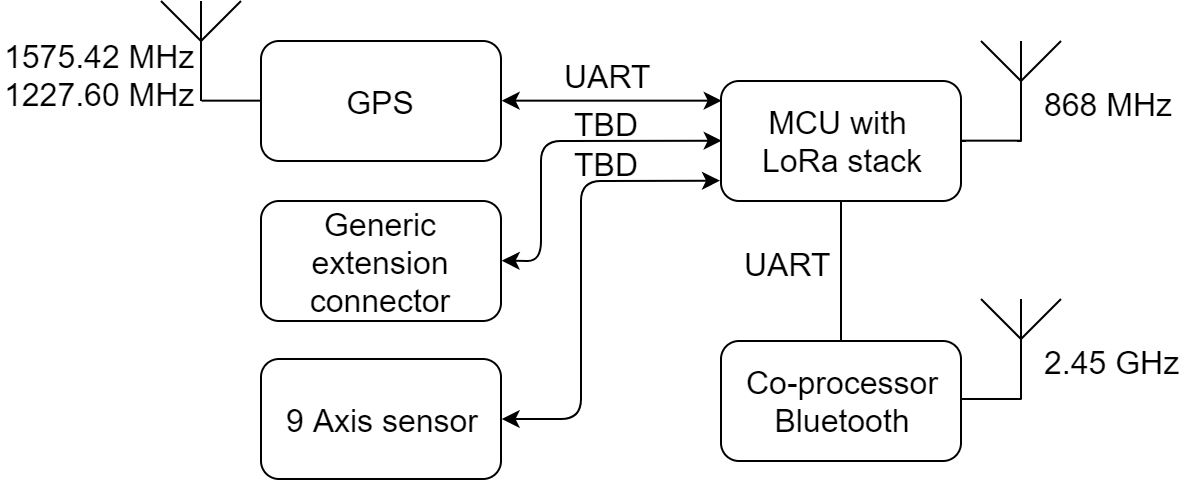
\includegraphics[width=\textwidth]{Figures/Hardware/master_onepage_option1.png}
    \caption{Architecture option numéro 1}
    \label{fig-hardware_option1}
\end{figure}

\begin{figure}[ht!]
    \centering
    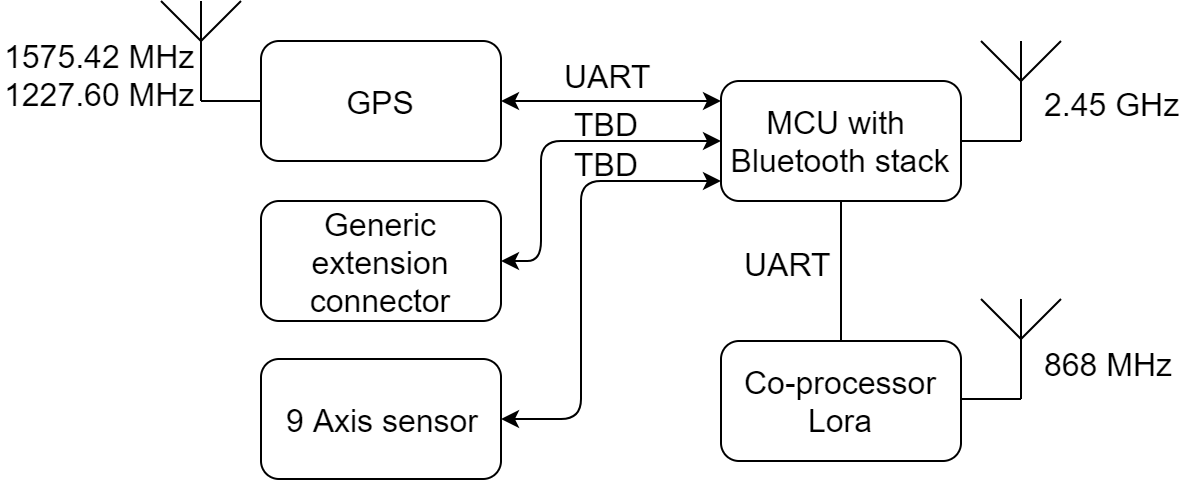
\includegraphics[width=\textwidth]{Figures/Hardware/master_onepage_option2.png}
    \caption{Architecture option numéro 2}
    \label{fig-hardware_option2}
\end{figure}

L'architecture choisie est l'option numéro 2. Nous avons donc tous les périphériques qui sont connectés au processeur s'occupant du Bluetooth. Le processeur avec l'interface LoRa, lui ne s'occupe, quant à lui, que de communiquer les évènements de réception de données et de transférer les messages provenant depuis le processeur Bluetooth. Il est également plus simple de faire une API pour le LoRa, le nombre de données et paramètres configurables étant moins important que dans le cas des communications Bluetooth. Si on souhaite faire une API entre les deux processeurs, il est ainsi nécessaire de tenir compte de la complexité de ceux-ci. Les accès LoRa sont également plus ponctuels. Le nombre de paquets envoyés par heures est très faible, en comparaison avec ce qui est réalisable en Bluetooth. On peut ainsi faire en sorte que le processeur soit en mode très basse consommation en attendant une commande de la part du processeur principal ou la réception d'un paquet LoRa sur son antenne.


\section{Choix des composants et leurs caractéristiques}

Cette section a pour but d'une part d'expliquer les différents choix effectués pour les composants présents sur la DevBox et, d'autre part, de présenter les caractéristiques principales des composants les plus importants.

\subsection{Microcontrôleur}
\label{subsect:microcontroleur}

Le microcontrôleur est le c\oe ur de ce projet; c'est dans celui-ci que la plus grande partie du développement va se produire. Il est dès lors important de sélectionner le composant idéal pour notre application, car une fois la sélection faite et les cartes électroniques réalisées, il est impossible de le changer sans générer des changements conséquents. Pour éviter cela, une étude des divers microcontrôleurs disponibles sur le marché a été réalisée.

\subsubsection{Critères de comparaison}
Le microcontrôleur a dû être choisi judicieusement en fonction du cahier des charges. Un comparatif, visible sur le \cref{tab-mcu_table}, a donc été effectué.  L'un des premiers points retenus est le type de protocoles qui sont supportés par le microcontrôleur. Le Bluetooth Low Energy étant un prérequis, il nous a été possible de procéder à un premier filtre, ce qui explique également que tous les microcontrôleurs affichés disposent de cette fonctionnalité. Néanmoins, le Bluetooth Low Energy s'accompagne de la norme 4.2, annoncée le 2 décembre 2014 \cite{Bluetoot59:online}, et de la norme 5.0, annoncée quant à elle le 16 juin 2016. Cette dernière n'était malheureusement pas encore parfaitement supportée par tous les fabricants de microcontrôleurs. Comme précédemment expliqué en \cref{sec_2_4_GHz}, une simple mise à jour logicielle permet de promouvoir un microcontrôleur en Bluetooth 5.0, du moins, en garantissant les fonctionnalités primordiales du protocole. Les microcontrôleurs affichés dans le tableau disposaient, en date du 1er octobre 2017, uniquement des fonctionnalités listées, ce qui ne signifie toutefois pas qu'elles ne peuvent pas s'agrandir avec le temps. \\

Après le Bluetooth, le deuxième type de protocole est le IEEE 802.15.4 \cite{IEEE802137:online}. Ce standard IEEE n'est pas un protocole en tant que tel, mais un modèle qui est respecté par plusieurs protocoles. Parmi les protocoles qui utilisent ce standard, on retrouve le ZigBee, WirelessHART, MiWi, SNAP, ou encore le Thread. Ce standard est de plus en plus utilisé pour la domotique. En effet, il permet de facilement créer des réseaux maillés permettant ainsi une grande couverture de l'habitation.\\

Enfin, un moyen de communication en dessous d'un gigahertz était également envisageable. Si le processeur supporte cela, ce peut être un avantage pour la réalisation de futurs \textit{use cases}. Néanmoins, la communication dans cette plage de fréquence a quelques désavantages, en commençant par la taille de l'antenne qu'il faut utiliser. La consommation du processeur est également affectée, pouvant atteindre jusqu'à 100 mA (cf. EFR32M datasheet). LoRa entre dans cette catégorie, mais seuls les processeurs fournis par Semtech peuvent implémenter la modulation. Ils ne sont, à l'heure actuelle, pas assez développés pour pouvoir être utilisés comme unique processeur gérant du 2.4 GHz avec en parallèle une interface LoRa (868 ou 433 MHz). \\

On a ensuite l'aspect consommation lors de l'émission qui entre en jeu. Afin d'être le plus proche possible en termes de comparaison entre les différents modèles, la consommation en émission a été retenue pour la fréquence de 2.4 GHz avec une puissance de 0 dBm en sortie. Plus cette consommation est faible, plus notre système aura la possibilité d'être autonome grâce à sa batterie. Finalement, les deux derniers points à retenir sont la taille des mémoires (RAM et Flash), qui selon leur taille nous permettent de faire un programme plus complexe, puis le coût à l'unité du microcontrôleur. Les prix ont été sélectionnés pour une seule unité sur le site d'achat Mouser\footnote{\url{http://www.mouser.ch/}} Suisse. \,

Davantage d'éléments auraient pu être pris en compte pour la comparaison, à l'instar des périphériques disponibles ou la possibilité d'avoir une matrice d'assignation des pins, utile lorsque l'on souhaite avoir des cartes modulables. Ce qui est primordial, c'est d'avoir au minimum une interface de communication série (SPI, I2C ou UART), étant précisé que tous ces microcontrôleurs en ont plusieurs de disponibles. Il convient également de prendre en considération la consommation du microcontrôleur, surtout dans les modes de sommeil. Celle-ci se trouve dans la même plage pour tous les microcontrôleurs listés, soit aux environs des 200\,\si{\micro}A avec une vitesse du microcontrôleur réduite au minimum, tous les périphériques désactivés et la persistance des données en RAM. Pour sortir de ces modes, le réveil émane habituellement d'une interruption matérielle, de sorte à pouvoir continuer à exécuter le code une fois sorti de veille. Vu que la carte de développement finale sera équipée d'un GPS, lequel sera le point principal de la consommation, cette donnée n'a pas été intégrée dans le tableau, bien qu'elle soit observée sur chaque microcontrôleur.\\

\begin{sidewaystable}[!ht]
\centering
\caption{Comparaison des microcontrôleurs envisagés pour le projet}
\begin{tabular}{|l|l|l|c|c|c|c|l|l|c|c|l|}
\hline
\multicolumn{1}{|c|}{\textbf{Manufacturer}} & \multicolumn{1}{c|}{\textbf{Model}} & \multicolumn{1}{c|}{\textbf{CPU}} & \textbf{\begin{tabular}[c]{@{}c@{}}BLE\\ 4.2\end{tabular}} & \textbf{\begin{tabular}[c]{@{}c@{}}BLE\\ 5.0\end{tabular}} & \textbf{\begin{tabular}[c]{@{}c@{}}IEEE\\     802.15.4\end{tabular}} & \textbf{\begin{tabular}[c]{@{}c@{}}Sub\\     1GHz\end{tabular}} & \multicolumn{1}{c|}{\textbf{\begin{tabular}[c]{@{}c@{}}Receive \\     Current\end{tabular}}} & \multicolumn{1}{c|}{\textbf{\begin{tabular}[c]{@{}c@{}}Transmit\\ Current \\ (@ 2.4Ghz, \\ @ 0dBm)\end{tabular}}} & \textbf{\begin{tabular}[c]{@{}c@{}}Flash/\\     SRAM\end{tabular}} & \textbf{\begin{tabular}[c]{@{}c@{}}Disponi-\\     bility\end{tabular}} & \multicolumn{1}{c|}{\textbf{Price}} \\ \hline
NXP & KW41Z & \begin{tabular}[c]{@{}l@{}}Cortex\\ M0+\\@ 48 MHz\end{tabular} & Yes & No & Yes & No & 6.8 mA & 6.1 mA & \begin{tabular}[c]{@{}c@{}}512 kB\\ / 128 kB\end{tabular} & Yes & 6.34 CHF \\ \hline
NXP & QN908x & \begin{tabular}[c]{@{}l@{}}Cortex\\ M4F\\@ 32 MHz\end{tabular} & Yes & Yes & No & No & 3.4 mA & 3.4 mA & \begin{tabular}[c]{@{}c@{}}512 kB\\ / 128 kB\end{tabular} & Yes & 5.87 CHF \\ \hline
\begin{tabular}[c]{@{}l@{}}Texas\\     Instrument\end{tabular} & CC2650 & \begin{tabular}[c]{@{}l@{}}Cortex\\ M3\\@ 48 MHz\\+ M0 for RF\end{tabular} & Yes & No & Yes & No & 6.2 mA & 6.8 mA & \begin{tabular}[c]{@{}c@{}}128 kB\\ / 20 kB\end{tabular} & Yes & 6.34 CHF \\ \hline
\begin{tabular}[c]{@{}l@{}}Texas\\     Instrument\end{tabular} & CC2640R2F & \begin{tabular}[c]{@{}l@{}}Cortex\\ M3\\@ 48 MHz\\+ M0 for RF\end{tabular} & Yes & Yes & No & No & 6.1 mA & 7.0 mA & \begin{tabular}[c]{@{}c@{}}128 kB\\ / 20 kB\end{tabular} & Yes & 6.34 CHF \\ \hline
\begin{tabular}[c]{@{}l@{}}Nordic \\     Semiconductor\end{tabular} & NRF52832 & \begin{tabular}[c]{@{}l@{}}Cortex\\ M4F\\@ 64 MHz\end{tabular} & Yes & Yes & No & No & 5.4 mA & 5.3 mA & \begin{tabular}[c]{@{}c@{}}512 kB\\ / 64 kB\end{tabular} & Yes & 5.51 CHF \\ \hline
\begin{tabular}[c]{@{}l@{}}Nordic \\     Semiconductor\end{tabular} & NRF52840 & \begin{tabular}[c]{@{}l@{}}Cortex\\ M4F\\@ 64 MHz\end{tabular} & Yes & Yes & Yes & No & N/A & N/A & \begin{tabular}[c]{@{}c@{}}1MB /\\     256 kB\end{tabular} & No & N/A \\ \hline
Silicon Labs & \begin{tabular}[c]{@{}l@{}}EFR32M\\ G12P433\\ F1024\end{tabular} & \begin{tabular}[c]{@{}l@{}}Cortex\\ M4F\\@ 38 MHz\end{tabular} & Yes & Yes & Yes & Yes & 9.3 mA & 9.5 mA & \begin{tabular}[c]{@{}c@{}}1MB /\\     256 kB\end{tabular} & Yes & 13.5 CHF \\ \hline
\end{tabular}
\label{tab-mcu_table}
\end{sidewaystable}


\subsubsection{Comparaisons et choix}
\label{sec-hardware_mcu_compare}

Pour une comparaison, il est nécessaire d'analyser les microcontrôleurs listés dans le \cref{tab-mcu_table}. Tout d'abord, le seul qui intègre tous les protocoles de communication est le Silicon Labs EFR32MG12P433F1024\footnote{\url{https://www.silabs.com/products/wireless/mesh-networking/efr32mg-mighty-gecko-zigbee-thread-soc/device.EFR32MG12P433F1024}}. En effet, celui-ci dispose de multiples interfaces et le support pour la dernière technologie Bluetooth. Il a tout pour son avantage excepté deux choses: son prix et sa consommation. Il est presque trois fois plus cher qu'un NRF52832, bien qu'au final ce prix soit compréhensif, puisque celui-ci supporte 2 protocoles supplémentaires. Vient ensuite la problématique de la consommation. Si l'on compare sa consommation à 2.4 GHz, elle est plus élevée que tous les microcontrôleurs présents sur le \cref{tab-mcu_table}. Si le projet nécessitait absolument l'utilisation de tous ces protocoles en parallèle, ce microcontrôleur serait alors le meilleur choix. Cela étant, c'est surtout le Bluetooth qui présente un intérêt pour le projet.\\

Le CC2650\footnote{\url{http://www.ti.com/product/CC2650}} du constructeur Texas Instruments est un microcontrôleur très utilisé dans le commerce, mais qui présente un défaut majeur, la taille de sa mémoire. En effet, ses 128 KB de flash et, surtout ses 20 kB de RAM, sont très limitatifs en termes de performances. Dans les besoins du projet, plusieurs tâches communiqueront en parallèle les unes avec les autres, avec des transferts de données qui engendreront des allocations mémoire diverses et conséquentes. Vient ensuite la création des données et l'utilisation de bibliothèques externes pour certains capteurs. Cela implique beaucoup de codes, en particulier si l'on se trouve dans une approche de prototypage où l'optimisation logicielle n'est pas forcément une priorité dès le départ. Le CC2650 et le CC2640R2F\footnote{\url{http://www.ti.com/product/CC2640R2F}} présentent tous deux cette problématique; ils sont équipés d'un dual processeur, d'un M3 pour l'application et d'un M0 pour la gestion des communications Bluetooth. L'avantage du CC2640R2F est qu'il supporte également le BLE 5.0 au détriment de l'IEEE 802.15.4. TI a d'ores et déjà annoncé qu'il ne prévoit pas de développement pour le BLE 5.0 sur le CC2650 \cite{CC2650Bl25:online}.\\

Il reste donc quatre microcontrôleurs qui semblent intéressants dans cette liste. Deux du fabricant NXP et deux du fabricant Nordic Semiconductor. Parmi ceux-ci, il y a le NRF52840, soit le microcontrôleur parfait pour notre application. Il est dans la même gamme de prix que ses concurrents et possède deux très grandes mémoires (flash et RAM). Il a comme avantage de supporter le Bluetooth et l'IEEE 802.15.4. Il est équipé d'un Cortex M4F à 64 MHz, ce qui fait de lui le processeur le plus performant parmi les sept du \cref{tab-mcu_table} (à égalité avec le NRF52832). Sa consommation n'étant pas encore connue au démarrage du projet, celle-ci n'a pas été spécifiée dans le tableau. Malheureusement, lorsque ce projet a commencé, le NRF52840 n'était disponible à la vente chez aucun fournisseur. La documentation du fabricant ne se résumait, à l'époque, qu'à une simple \textit{datasheet} minimaliste, sans aucun guide utilisateur complet. À l'heure de la rédaction de ce rapport (janvier 2018), une version BGA 125 pins est disponible, malheureusement avec quelques mois de retard pour notre application. Malgré le fait que ce microcontrôleur soit en BGA, il s'agit là certainement de l'un des meilleurs choix pour une application Bluetooth. La version NRF52832 a des caractéristiques identiques au NRF52840, excepté le fait qu'il ne supporte que du Bluetooth Low Energy.\\

NXP offre également plusieurs microcontrôleurs dans la gamme de fréquences 2.4GHz qui sont orientés basse consommation. Les deux plus intéressants sont le QN908x et le KW41Z. Le KW41Z est équipé d'un CPU Cortex-M0+ de ARM alors que le QN908x est quant à lui pourvu d'un M4F. Malgré un M0+, le KW41Z a comme atout le fait de pouvoir supporter la spécification IEEE 802.15.4 et, surtout, le protocole Thread précédemment présenté dans la \cref{sec-thread_protocol}. Ces deux protocoles peuvent être utilisés en parallèle, ouvrant ainsi la possibilité de créer des ponts entre ces deux mondes. \\


En somme, le choix s'articule autour du NRF52832 et du KW41Z. Finalement, le microcontrôleur retenu a été le KW41Z de NXP. Celui-ci a été initialement développé par l'entreprise Freescale, qui depuis le développement de ce produit a été rachetée par NXP. Un argument intéressant est le fait que le KW41Z puisse être connecté à la fois un réseau Bluetooth LE et à un réseau IEEE 802.15.4. Sa connectivité à un réseau Thread est également un avantage si l'on souhaite utiliser la carte dans un milieu plus \textit{SmartHome} que \textit{SmartCities}. Bien qu'il n'utilise qu'un Cortex-M0 de ARM, pour le type d'application que l'on souhaite réaliser, la puissance de calcul n'est pas le prérequis le plus important. C'est donc le KW41Z qui a été retenu pour ce projet. 

\FloatBarrier
\subsubsection{NXP Kinetis KW41Z}
\label{sec-hardware_kw41z}

La \cref{fig-KW41Z_block_diagram} illustre le contenu du KW41Z avec tous ses composants internes. On remarque des éléments intéressants dans la section \textit{security}, soit un support de chiffrement AES-128 et la possibilité de générer des nombres aléatoires avec un \textit{True Random Number Generator} (TRNG). Ces deux éléments ne visent pas un but précis dans le cadre des applications présentées dans ce projet, mais si l'utilisateur souhaite un grand niveau de sécurité, il a la possibilité d'accéder à ces deux éléments.\\


\begin{figure}[ht!]
    \centering
    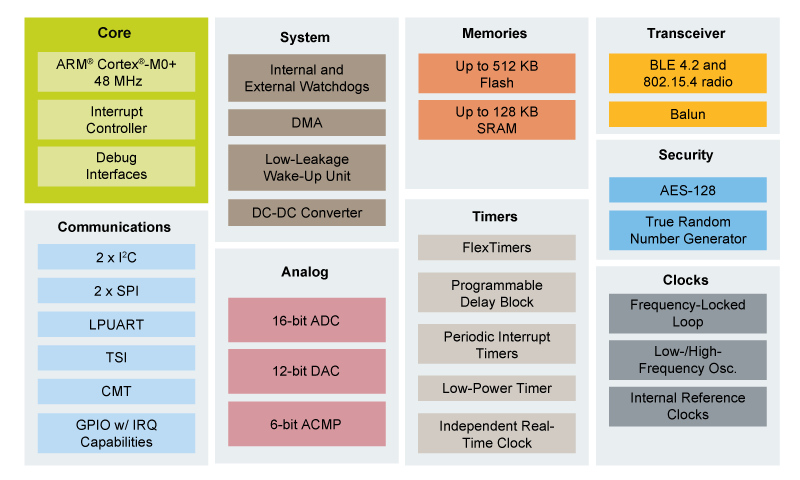
\includegraphics[width=\textwidth]{Figures/Hardware/KW41Z_block_diagram.jpg}
    \caption{Diagramme bloc interne du KW41Z}
    \label{fig-KW41Z_block_diagram}
\end{figure}

Une fois le microcontrôleur choisi, il était nécessaire de déterminer, les types d'interfaces allant être utilisées pour les différentes communications sur la DevBox. On peut voir sur \cref{fig-KW41Z_block_diagram} la présence de deux interfaces I2C, de deux SPI et d'une LPUART. Celle en UART a été réservée pour la communication entre le microcontrôleur Bluetooth et le coprocesseur LoRa. L'UART offre l'implémentation la plus versatile dans ce type de communication. Il peut y avoir des messages asynchrones provenant du coprocesseur selon le type de protocole de communication que l'utilisateur souhaite utiliser entre les deux éléments. Des interfaces SPI et I2C sont utilisées par les composants inclus sur la carte électronique. Cette même interface SPI est partagée avec un connecteur PMOD installé sur la DevBox. Une deuxième interface I2C est quant à elle réservée au port PMOD. Pour une vue d'ensemble des interfaces de communication et leurs connexions sur la carte DevBox, il est conseillé de visualiser le schéma Altium en \cref{AppendixDevBoxHardware}, sur le schéma nommé \texttt{Top View}.\\

\begin{figure}[ht!]
    \centering
    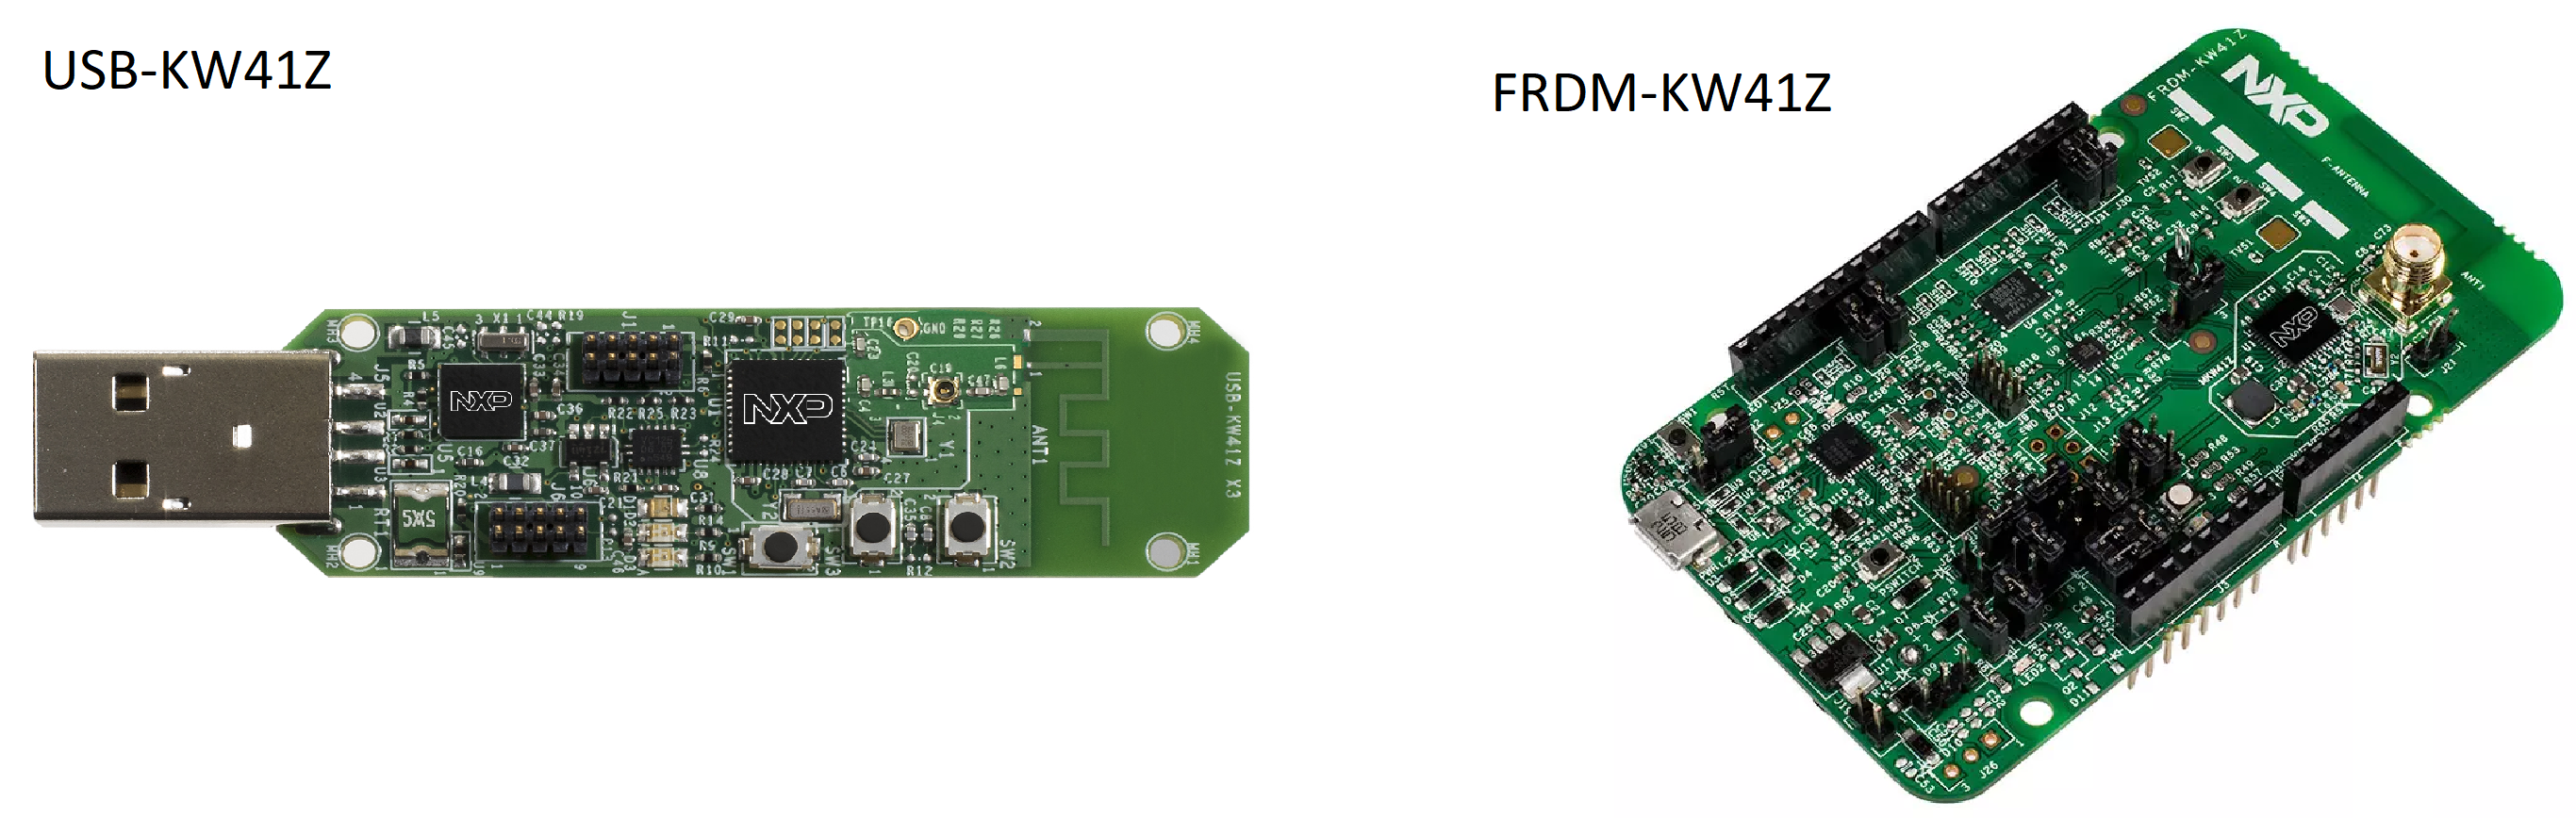
\includegraphics[width=\textwidth]{Figures/Hardware/nxp_dev_boards.png}
    \caption{Cartes de développement pour KW41Z}
    \label{fig-nxp_dev_boards}
\end{figure}

NXP propose deux cartes de développement avec le KW41Z visibles sur la \cref{fig-nxp_dev_boards}. La première est un simple dongle USB avec quelques boutons et une LED qui peut s'avérer utile pour faire des tests, par exemple, si on a besoin de scanner des paquets Bluetooth Low Energy. La FRDM-KW41Z est beaucoup plus complète. Elle propose en premier lieu des connecteurs compatibles avec les cartes d'extension Arduino. Elle contient en outre une meilleure antenne sur le PCB avec la possibilité de faciliter la connexion d'une antenne externe sur le connecteur prévu à cet effet. La carte est également équipée d'une vingtaine de \textit{jumpers} qui offrent la possibilité de tester les différents modes de consommation du circuit, ainsi que plusieurs confirmations des sorties. Elle possède également une mémoire flash externe qui peut être utilisée pour les mises à jour OTAA, ainsi qu'un accéléromètre/gyroscope via l'intégration d'un FXOS8700CQ. Cette deuxième carte a été utilisée dans le cadre de ce projet pour avoir une première approche avec les outils de programmation et ainsi pouvoir commencer à programmer parallèlement à la réalisation du PCB.


\FloatBarrier
\subsection{Gestion de la batterie}

Le système doit pouvoir être autonome. Afin de garantir cela, une batterie peut être connectée. La capacité de cette batterie reste au choix de l'utilisateur. 
L'utilisateur peut recharger celle-ci à l'aide d'un connecteur micro-USB présent sur la carte. L'aspect autonomie peut être encore plus poussé en connectant un panneau solaire directement sur la carte. Celui-ci a son propre connecteur dédié en entrée. Ce panneau permet ainsi de directement charger la batterie qui fournira à son tour la tension pour le système. 

Pour optimiser le rendement lors de l'utilisation d'un panneau solaire, un circuit intégré nommé BQ24210 \footnote{\url{http://www.ti.com/product/BQ24210}} a été utilisé. Ce dernier s'occupe directement de la recharge de la batterie supportant en entrée jusqu'à 20V de tension. Il est capable de fournir jusqu'à 800\,mA à la batterie, tout en protégeant celle-ci en cas de surtension. Il accepte également la possibilité de recharger avec une tension de 5V, permettant ainsi la recharge directement depuis une prise USB. \\


Une batterie est couplée au système. Celle-ci n'a pas de restriction de taille, elle doit simplement être de type Li-Ion en raison de la tension et de la courbe de charge fournie par le BQ24210. La batterie n'a pas besoin d'offrir un circuit de protection contre les surcharges ni les décharges profondes. Comme expliqué précédemment, le circuit BQ24210 interrompt la charge lorsque la batterie est pleine et protège la batterie des décharges profondes.  \\

L'ensemble de la carte est alimentée en 3.3V à l'aide d'un régulateur TPS62291. Celui-ci peut fournir un courant maximum de 1A. Ce haut courant est une précaution selon le type de cartes d'extensions que l'utilisateur souhaite ajouter à la DevBox. Il dispose d'un courant typique de fonctionnement très faible de 15 µA, pouvant ainsi consommer un minimum si l'on souhaite mettre toute la carte en basse consommation.

\FloatBarrier
\subsection{Coprocesseur LoRa}

La communication via LoRa est uniquement possible en utilisant les circuits proposés par l'entreprise Semtech, laquelle propose une gamme de circuits qui est visible à l'adresse suivante : 
\begin{center}
    \url{{http://www.semtech.com/wireless-rf/lora.html}}
\end{center}

Tous les circuits intégrés proposés sur le site de Semtech sont des périphériques qu'il faut ensuite relier avec un microcontrôleur via une communication SPI. Afin de pallier à cela, plusieurs fabricants ont développé des circuits intégrés composés d'un processeur couplé à un module de Semtech. Cela permet ainsi d'économiser du temps de conception. En effet, le plus difficile dans l'intégration de ces modules est la gestion de la partie radiofréquence. Celle-ci nécessite souvent des composants spécifiques qui supportent des fréquences plus élevées que des composants traditionnels. C'est le cas des condensateurs et inductances utilisées, ceux-ci devant être indiqués par le fabricant comme étant utilisables pour des fréquences supérieures à plusieurs gigahertz. Le plus souvent, les fabricants proposent des gammes complètes de ces composants pour ces cas d'utilisations, à l'instar des fabricants Murata\footnote{\url{https://www.murata.com/tool/netlist/mlcc}} ou Vishay\footnote{\url{https://www.vishay.com/capacitors/high-frequency/}}. \\

\begin{figure}[ht!]
    \centering
    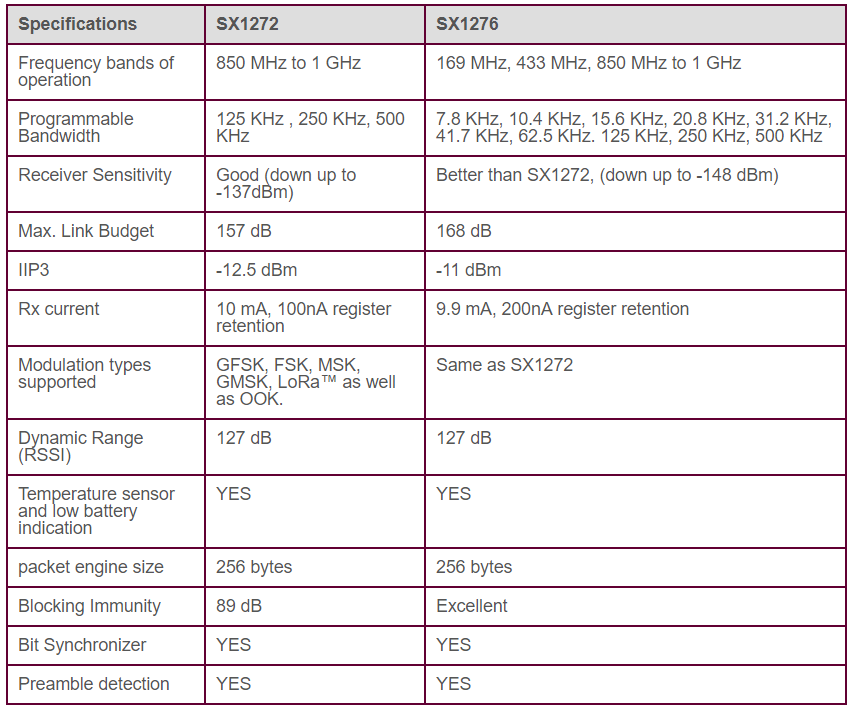
\includegraphics[width=0.9\textwidth]{Figures/Hardware/sx1272_vs_sx1276.PNG}
    \caption{Comparatif SX1272 et SX1276}
    \label{fig-sx1272_vs_sx1276}
\end{figure}

Tous les modules sont équipés d'un processeur connecté via SPI avec un circuit de Semtech. Parmi ces circuits se trouvent le SX1272 et le SX1276. Un comparatif sur le site \texttt{rfwireless-world}\footnote{\url{http://www.rfwireless-world.com/Terminology/SX1272-vs-SX1276-Semtech-LoRa-RF-Transceivers.html}} offre une vue d'ensemble des différences entre ces deux circuits. La \cref{fig-sx1272_vs_sx1276} illustre cette comparaison. Ils sont similaires, mais le SX1276 offre de meilleures performances. En effet, on constate que le SX1276 propose davantage de bandes fréquence ainsi qu'un meilleur \textit{link budget} (correspondant à la puissance de réception\footnote{\url{https://en.wikipedia.org/wiki/Link_budget}}). Le SX1272 ne propose que la fréquence 868 et 915 MHz de la bande de fréquence LoRa, soit celle respectivement pour l'Europe et l'Amérique du Nord respectivement. L'Asie avec ses 433 MHz n'est donc pas supportée. Le SX1276 est actuellement l'une des meilleures options disponibles par Semtech pour connecter un n\oe ud à un réseau LoRaWAN. Néanmoins, pour notre application, le SX1272 est parfaitement suffisant.\\

En termes de consommation, les deux circuits sont similaires. Preuve en est la comparaison des données présentes dans leurs \textit{datasheets} respectives (cf. \cref{fig-sx1272_78_current_consumption}). Dans le cadre d'applications low power, les consommations en veille et au repos sont les plus importantes. Celles-ci sont de 0.1 ou 0.2\,\si{\micro}A pour le mode \textit{sleep} et de 1.5\,\si{\micro}A pour le mode \textit{idle}. Ils constituent des circuits parfaits pour des applications basse consommation. Qui plus est, si on émet à la puissance maximale de 20 dBm, la consommation peut monter à 128 mA dans le cas du SX1272, constat qui doit être pris en compte lors du dimensionnement de l'alimentation du système.

\begin{figure}[ht!]
    \centering
    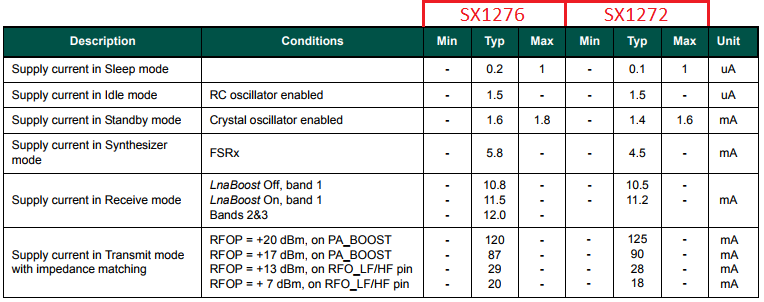
\includegraphics[width=0.9\textwidth]{Figures/Hardware/sx1272_78_current_consumption.PNG}
    \caption{Comparaison de la consommation de courant entre le sx1272 et sx1278}
    \label{fig-sx1272_78_current_consumption}
\end{figure}


\FloatBarrier
\subsubsection{Murata CMWX1ZZABZ-078}
\label{sec-hardware_lora_module}
\begin{figure}[ht!]
    \centering
    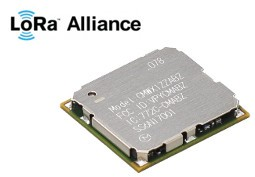
\includegraphics[width=0.4\textwidth]{Figures/Hardware/murata_module_image.jpg}
    \caption{Module LoRa CMWX1ZZABZ-078}
    \label{fig-murata_module_image}
\end{figure}

Le célèbre fabricant de semiconducteurs Murata\footnote{\url{https://www.murata.com/}} a commercialisé, en juillet 2016,  un module LoRa intégrant un SX1276, ainsi qu'un processeur de STMicroelectronics \cite{Muratala5:online}. Le module est visible sur la \cref{fig-murata_module_image}. Murata est renommé pour ses composants passifs de très haute précision, comme ses résistances, condensateurs ou inductances. Comme expliqué dans la section précédente, c'est toujours un challenge d'optimiser des circuits lorsque l'on utilise de hautes fréquences. Murata a développé ce circuit en y ajoutant ses composants afin d'offrir les meilleures performances en radio fréquence tout en minimisant l'espace occupé sur un PCB par le module.\\

\begin{figure}[ht!]
    \centering
    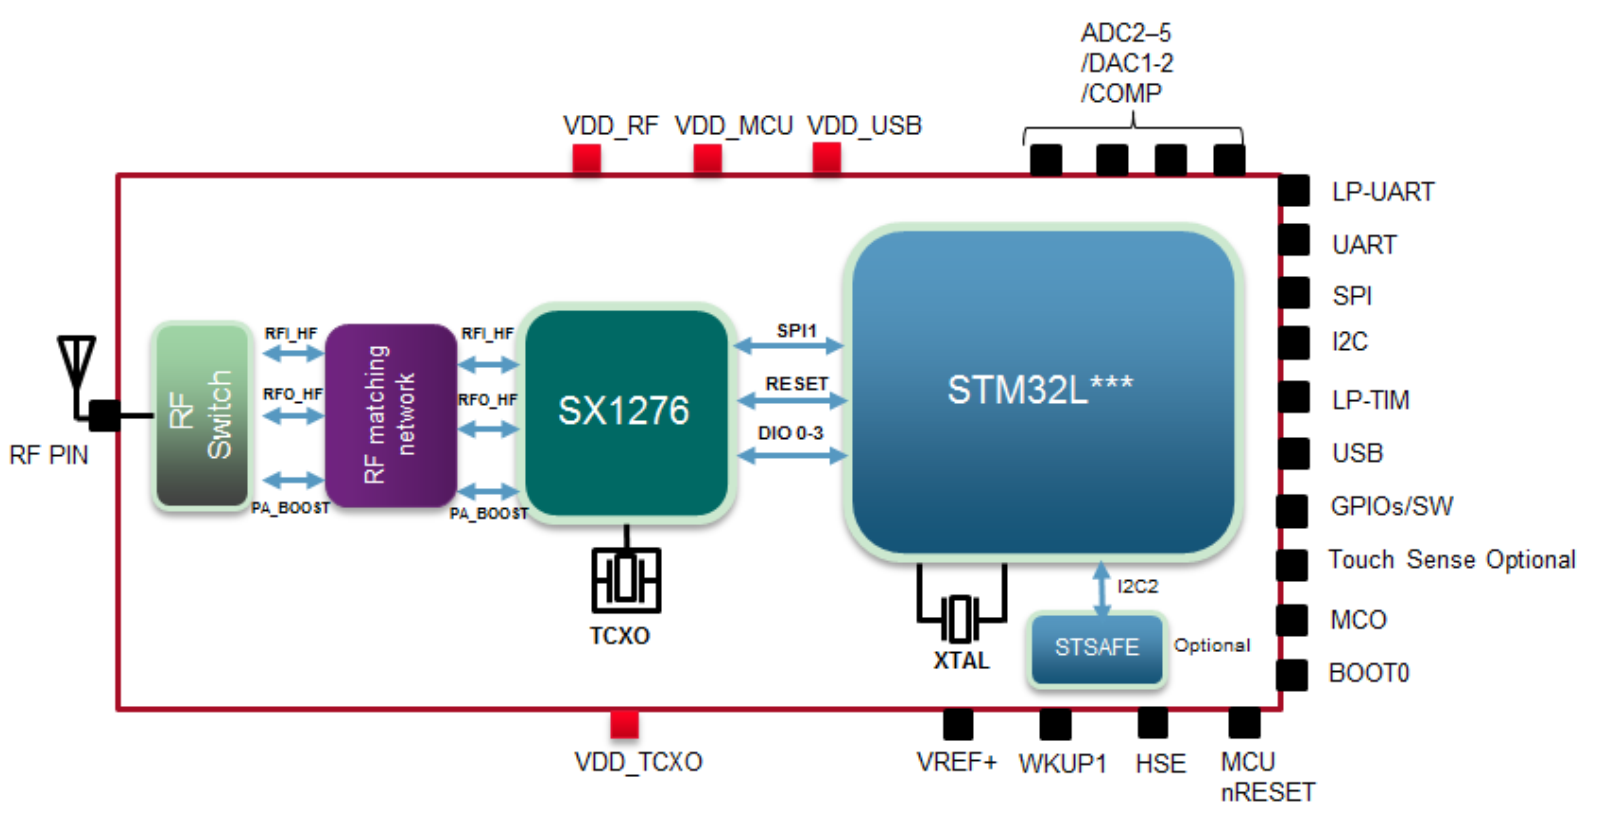
\includegraphics[width=0.9\textwidth]{Figures/Hardware/murata_bloc_diagram.PNG}
    \caption{Contenu du module LoRa CMWX1ZZABZ-078}
    \label{fig-murata_bloc_diagram}
\end{figure}

La \cref{fig-murata_bloc_diagram} illustre le contenu interne du module. On peut y voir un processeur ainsi que le SX1276. Le point fort de ce module est toutefois l'électronique placée entre le SX1276 et l'antenne. En effet, c'est la partie la plus difficile à réaliser lorsque l'on fait du routage haute fréquence, puisqu'il faut adapter les impédances et le dimensionnement des composants. Il existe en réalité deux modèles du CMWX1ZZABZ, la version 078 et la 091. La différence entre les deux est le processeur ST qui est placé en interne. Le 078 contient un STM32L082 alors que le 091 est équipé du STM32L072. C'est de là d'où proviennent les astérisques sur la \cref{fig-murata_bloc_diagram} avec le bloc bleu représentant le processeur. Cependant, à l'heure actuelle, le CMWX1ZZABZ-078 est le seul disponible sur le marché, aucun revendeur ne propose l'autre alternative. La \cref{fig-murata_bloc_diagram} nous indique également la présence d'un composant nommé \cref{sec-mcu_stsafe}. Son nom complet est \textit{State-of-the-art security for peripherals and IoT devices}. Celui-ci est développé par STMicroelectronics et propose plusieurs mécaniques d'authentification, afin de garantir que le périphérique fournissant des données à un client n'a pas été usurpé par une entité tierce. Ce périphérique est exploré plus en détail dans la \cref{sec-mcu_stsafe}.\\

Ses dimensions sont de 12.5\,mm x 11.6\,mm x 1.76\,mm; il est le plus petit des modules présentés ici. Ceci vient surtout du fait que Murata a utilisé sur son circuit des composants passifs avec des boitiers 0201 et 01005, ce qui lui a permis de créer le module le plus compact possible. C'est le seul des modules listé dans ce document qui propose un SX1276, contrairement à ses concurrents qui utilisent un SX1272. \\

La \textit{datasheet} du module ne spécifie pas toutes les consommations en courant. La \cref{fig-murata_current_consumption} contient le peux d'informations qui sont disponibles sur ses consommations. On y retrouve la consommation maximale du composant lors de l'émission à 20dBm. La \textit{datasheet} indique l'ajout de 3 mA en comparaison avec à la consommation seule du SX1276 (cf. \cref{fig-sx1272_78_current_consumption} pour les diverses consommations). Concernant la consommation en \textit{sleep}, on peut observer celle du STM32L082 pour avoir une idée, puisqu'aucune estimation n'est fournie par Murata. La \cref{fig-stm32L0_current_consumption} montre la consommation d'un STM32L082 en mode \textit{low power} avec tous les périphériques éteints. Ce mode serait envisageable avec la DevBox, car le microcontrôleur Bluetooth est capable d'activer ce mode à l'aide, par exemple, d'un GPIO. On observe des consommations très faibles en fonction des horloges choisies. Dans l'ensemble, la consommation du processeur varie de 4.7\,\si{\micro}A à 73\,\si{\micro}A selon la fréquence désirée et de la température d'opération. Il faut ensuite ajouter les consommations du SX1276 dans un mode similaire. Les consommations du SX1276 ont été précédemment présentées dans la \cref{fig-sx1272_78_current_consumption}, laquelle indiquait une consommation en mode \textit{sleep} de 0.2\,\si{\micro}A. Ce sont des courants tout à fait adaptés à des applications basse consommation. \\

\begin{figure}[ht!]
    \centering
    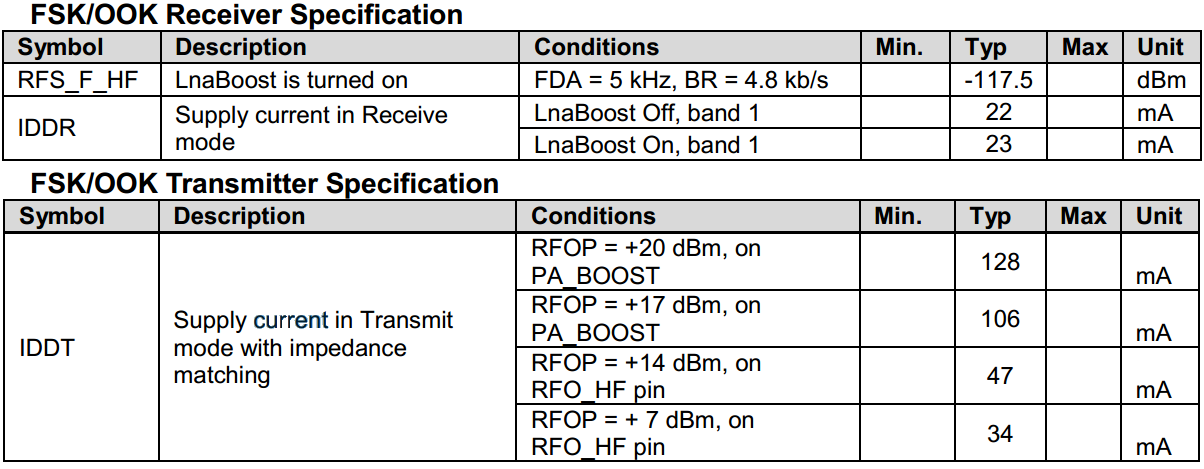
\includegraphics[width=0.9\textwidth]{Figures/Hardware/murata_current_consumption.PNG}
    \caption{Consommation en courant du module CMWX1ZZABZ-078}
    \label{fig-murata_current_consumption}
\end{figure}

\begin{figure}[ht!]
    \centering
    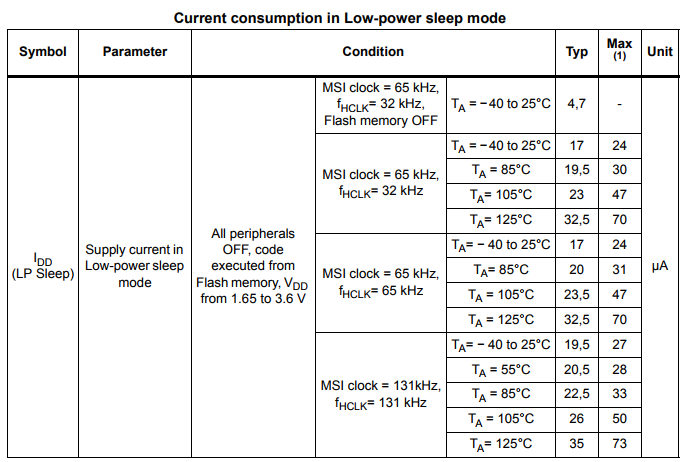
\includegraphics[width=0.9\textwidth]{Figures/Hardware/stm32L0_current_consumption.PNG}
    \caption{Consommation en courant du microcontrôleur STM32L082}
    \label{fig-stm32L0_current_consumption}
\end{figure}


\FloatBarrier
\subsubsection{IMST iM880B}

\begin{figure}[ht!]
    \centering
    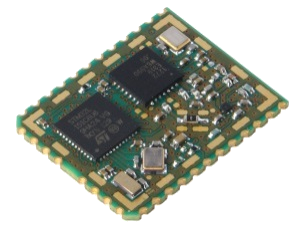
\includegraphics[width=0.7\textwidth/2]{Figures/Hardware/im880b-l_lora_module.png}
    \caption{Module LoRa iM880B du fabricant IMST}
    \label{fig-im880b-l_lora_module}
\end{figure}

Le module iM880B, visible sur la \cref{fig-im880b-l_lora_module}, est un produit de l'entreprise IMST. Celle-ci est renommée pour ses concentrateurs LoRa nommés iC880A\footnote{\url{https://wireless-solutions.de/products/radiomodules/ic880a.html}} qui, dotés d'un prix très accessible, facilitant la mise en place d'une gateway LoRaWAN. \\

Sa dimension étant de 25 x 20\,mm, il presque quatre fois plus grand que le module de Murata. Il dispose toutefois d'un processeur plus puissant que le Murata. En effet, il s'agit là de la gamme STM32L1, contrairement au STM32L0 du CMWX1ZZABZ. Le STM32L1 est basé sur un Cortex M3 cadencé à 16 MHz. Un processeur puissant n'a pas vraiment de sens dans ce projet, car le processeur LoRa restera le plus clair de son temps en veille en attendant des commandes du processeur principal.\\

\begin{figure}[ht!]
    \centering
    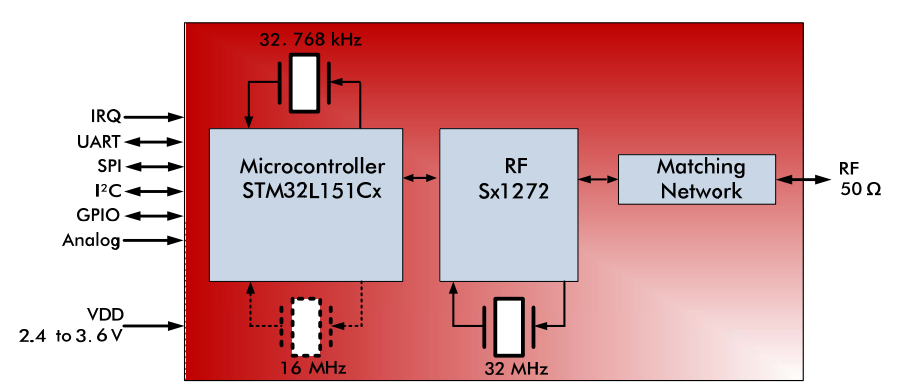
\includegraphics[width=0.7\textwidth]{Figures/Hardware/imst_bloc_diagram.PNG}
    \caption{Contenu du module LoRa iM880B}
    \label{fig-imst_bloc_diagram}
\end{figure}

La \textit{datasheet} de ce module nous fournit plus d'informations sur sa consommation. Les consommations sur les multiples modes sont visibles sur la \cref{fig-imst_current_consumption}. On a la même consommation en émission maximale que le Murata à 128 mA à +20 dBm. Cette \textit{datasheet}, présente cette fois la consommation lorsque le périphérique est en mode \textit{low power}. Celle-ci s'élève à 1.85\,\si{\micro}A avec un RTC activé, ou 800 nA sans celui-ci. La consommation du STM32L082 est donc similaire à celle du Murata. Malgré l'utilisation d'un processeur plus puissant (STM32L1), la consommation est donc inférieure à celle du CMWX1ZZABZ (4.9\,\si{\micro}A). Il faudrait examiner quel mode du microcontrôleur est activé dans cette configuration pour pouvoir faire une comparaison exacte entre les deux configurations. Dans le cas du Murata, il s'agissait du mode \textit{sleep} du processeur, mais cette information n'est pas disponible pour le module IMST.\\

\begin{figure}[ht!]
    \centering
    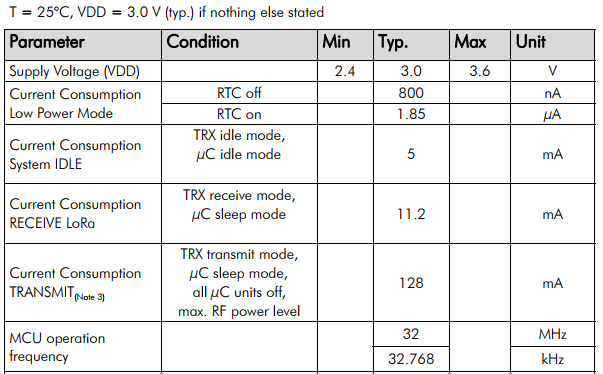
\includegraphics[width=0.7\textwidth]{Figures/Hardware/imst_current_consumption.PNG}
    \caption{Consommation en courant du module iM880B}
    \label{fig-imst_current_consumption}
\end{figure}

\FloatBarrier
\subsubsection{USI WM-SG-SM-42}

Le fabricant chinois USI a annoncé la production, en décembre 2016, d'un module similaire à celui de Murata. Celui-ci est nommé WM-SG-SM-42 et est visible sur la \cref{fig-usi_en.i-nucleo-lrwan1}. Celui-ci a été adopté par STMicroelectronics pour la création d'un \textit{shield} pouvant être placé sur des plateformes Arduino ou, directement, sur certaines de leur cartes de développement. Le contenu du module est illustré sur la \cref{fig-usi_bloc_diagram}.\\


\begin{figure}[ht!]
    \centering
    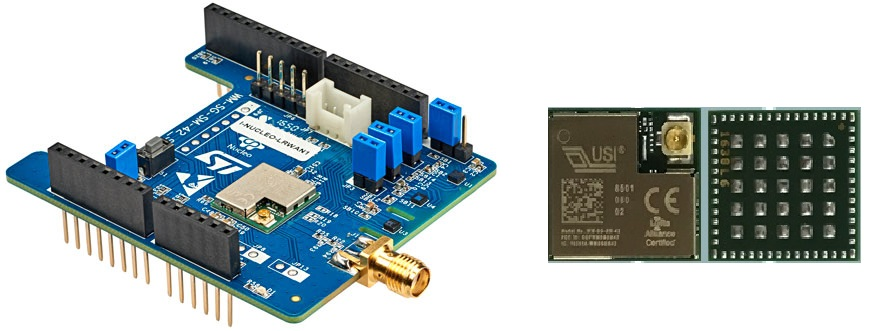
\includegraphics[width=0.75\textwidth]{Figures/Hardware/usi_i-nucleo-lrwan1.jpg}
    \caption{\textit{Shield} I-NUCLEO-LRWAN1 de ST et module USI WM-SG-SM-42}
    \label{fig-usi_en.i-nucleo-lrwan1}
\end{figure}

\begin{figure}[ht!]
    \centering
    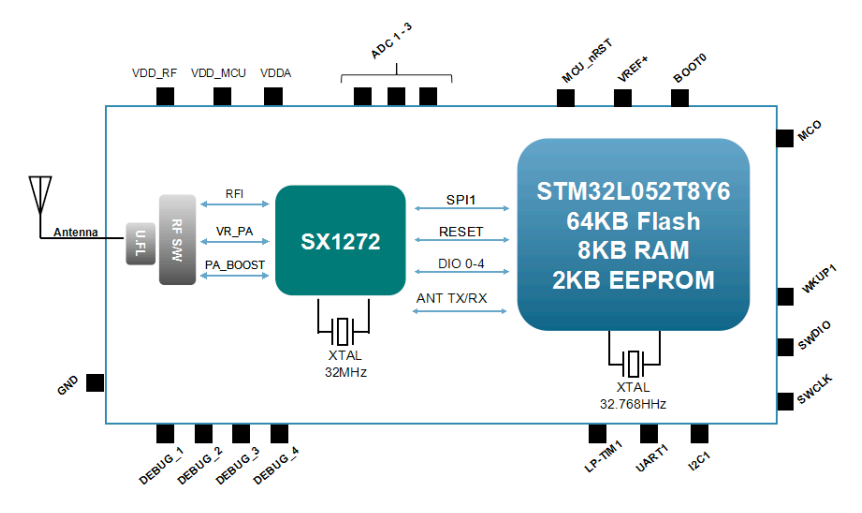
\includegraphics[width=0.8\textwidth]{Figures/Hardware/usi_bloc_diagram.PNG}
    \caption{Contenu du module WM-SG-SM-42}
    \label{fig-usi_bloc_diagram}
\end{figure}

Néanmoins, lorsque ce projet a commencé (septembre 2017), très peu d'informations étaient disponibles sur ce module, la seule référence postée sur le site du fabricant étant le communiqué de presse suivant : 
\begin{center}
    \url{http://www.usish.com/english/pressroom_more.php?n_sn=23}
\end{center}
Il n'y avait pas de description du produit ni de \textit{datasheet}, et le site n'était pas encore entièrement traduit en anglais. Il semble que tout cela se soit amélioré à la date de la rédaction de ce rapport (janvier 2018). Une page du produit est maintenant disponible\footnote{\url{http://www.usish.com/english/products_WM_SG_SM_42.php}}, de même qu’un PDF contenant une \textit{datasheet} du module\footnote{\url{http://www.usish.com/pdf/WM-SG-SM-42_Product\,\%20SPEC.pdf}}. Cependant, un problème majeur est toujours présent: ce module ne semble être disponible chez aucun revendeur; même sur des sites de vente en ligne comme Alibaba ou Aliexpress. Contrairement au module de Murata, qui est très facilement accessible. En revanche, le \textit{shield} produit par STMicroelectronics, équipé du module USI, est bien commercialisé en Europe et disponible chez plusieurs fournisseurs\footnote{\url{https://www.findchips.com/search/I-NUCLEO-LRWAN1}}.\\


Le module a une dimension de 12\,mm x 13\,mm, similaire au module de Murata. Il possède en outre un connecteur U.FL placé sur le module. Ceci est un avantage, puisqu'il permet d'économiser de la place sur le circuit si le but final est d'utiliser une antenne externe au PCB. Dans le cadre de ce projet, les deux options ont été retenues. L'utilisation de ce module aurait présenté un avantage en termes de gain de place. \\

\begin{figure}[ht!]
    \centering
    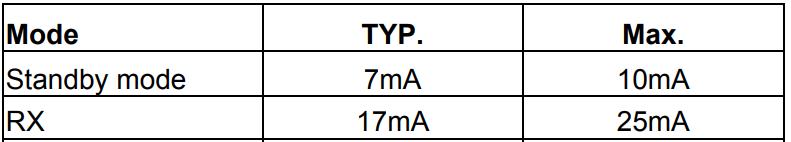
\includegraphics[width=0.7\textwidth]{Figures/Hardware/usi_current_consumption.PNG}
    \caption{Consommation en courant du module WM-SG-SM-42}
    \label{fig-usi_current_consumption}
\end{figure}

En ce qui concerne la consommation, la \textit{datasheet} reste très vague sur les informations. On peut voir uniquement les deux valeurs affichées sur la \cref{fig-usi_current_consumption} sur une configuration LoRa à 3.3V, 25°C et BW 125kHz. La consommation en mode \textit{standby} est trop élevée pour qu'elle soit celle de la consommation définitive du circuit. Il est possible de le mettre en mode \textit{low power}, mais la consommation de ce mode n'est pas documentée dans la \textit{datasheet}. Les consommations en émissions sont listées dans la \textit{datasheet} en fonction de la puissance d'émission. Elles varient de 47 mA à 126 mA à 868 MHz, avec des puissances d'émission allant de 5.6 à 19 dBm. Il faut être conscient que ces consommations ne sont présentes que lorsque l'utilisateur émet des paquets sur le réseau, sont durant quelques centaines de millisecondes au maximum. Pour la consommation en veille, on peut estimer que celle-ci est identique au Murata, puisque toute la gamme STM32L0 a des consommations similaires.\\

Comme pour les deux autres modules, la partie RF est intégrée dans le module, ce qui simplifie le développement matériel final. Il suffit de raccorder une antenne avec une impédance correcte de 50\,Ohms.

\subsubsection{Module choisi}

Le module de Murata est celui qui a été retenu pour ce projet. Il a l'avantage d'être extrêmement compact et simple à intégrer. Il est également disponible chez tous les revendeurs en Europe, contrairement à son rival, celui du fabricant USI. Au niveau logiciel, plusieurs codes exemples sont directement fournis par ST sur leur site Internet, ce qui offre un support en cas de problèmes au fil du développement.\\

\begin{figure}[ht!]
    \centering
    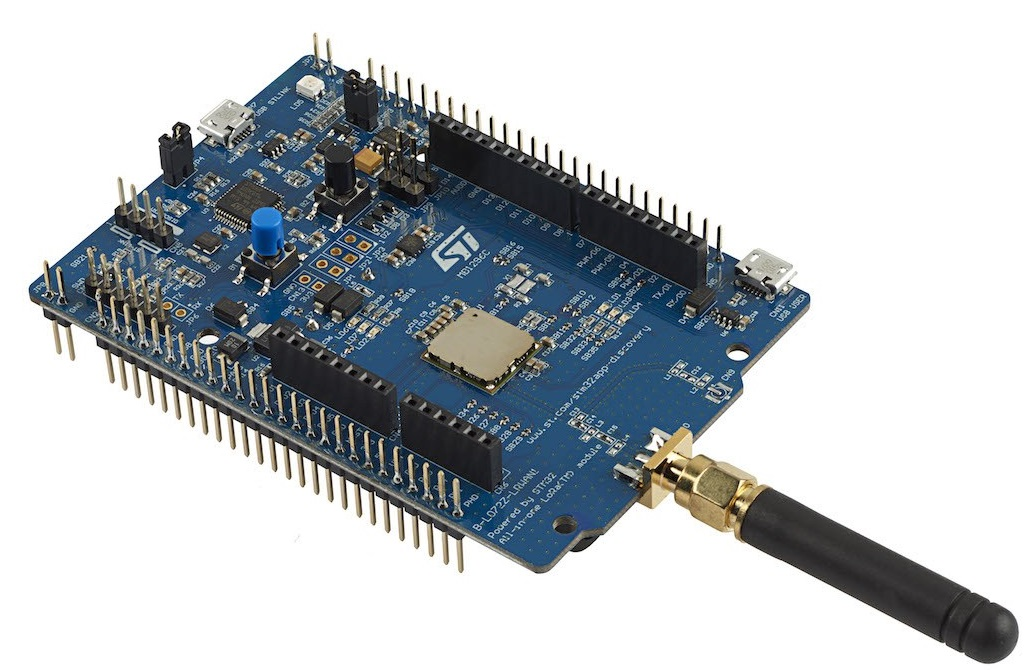
\includegraphics[width=0.6\textwidth]{Figures/Hardware/B_L072Z_st_dev_board.jpg}
    \caption{Carte de développement ST B-L072Z-LRWAN1}
    \label{fig-B_L072Z_st_dev_board}
\end{figure}

La carte de développement B-L072Z-LRWAN1 de ST Microelectronics, visible sur la \cref{fig-B_L072Z_st_dev_board}, offre la possibilité directement commencer à travailler sur le matériel sans que la carte électronique ne soit finalisée. Une partie du code de cette carte peut ensuite être facilement adapté sur la DevBox.



\subsection{Périphériques}

La carte DevBox est équipée de certains périphériques capteurs de données. Cette sous-section a pour but de les énumérer et de présenter leurs principales caractéristiques. Le schéma contenant ces périphériques est disponible dans l'\cref{AppendixDevBoxHardware} de ce document. Ils sont principalement présentés dans les schémas nommés \texttt{Embedded Sensors}, \texttt{GPS} et \texttt{PMOD}.

\subsubsection{LED}

Chaque microcontrôleur a à sa disposition quatre LED. Une bleu, une verte, une rouge ainsi qu'une jaune. Ces LED sont contrôlables via des GPIOs avec un état bas pour les allumer. Elles sont programmables selon la volonté de l'utilisateur.

\subsubsection{Buttons}

Chaque microcontrôleur a à sa disposition 2 boutons poussoirs. Ceux-ci produisent un état bas sur les GPIOs lorsque le bouton est pressé. Ces boutons sont programmables selon la volonté de l'utilisateur.

\subsubsection{Plateforme inertielle 9 axes}

\begin{figure}[ht!]
    \centering
    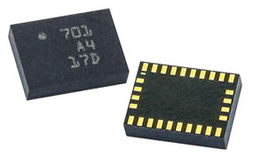
\includegraphics[width=0.35\textwidth]{Figures/Hardware/bno055_model.png}
    \caption{Plateforme 9 axes BNO055}
    \label{fig-bno055_model}
\end{figure}

La DevBox dispose d'une plateforme inertielle 9 axes (14-bit accéléromètre, 16-bit gyroscope et 16-bit magnétomètre) intégrés dans un même circuit électronique. Il s'agit du BNO055 fabriqué par Bosch Sensortec, visible sur la \cref{fig-bno055_model}, dont la communication s'effectue via un bus I2C relié au processeur principal (KW41Z). L'adresse I2C est configurable en fonction de l'état de la pin COM3 du module. Deux résistances (R11 et R13, une seule doit être placée) permettent de choisir le dernier bit de l'adresse. Si la résistance R11 est placée, le périphérique comporte alors l'adresse 0x29. Si c'est la résistance R13, cette adresse est 0x28. \\

À l'intérieur de ce composant, on trouve un ARM Cortex-M0+ avec un \textit{firmware} développé par Bosch, afin de pouvoir délocaliser le calcul de certaines données capturées. Cela permet, par exemple, de demander au composant de retourner la valeur de la gravité en $m/s^2$ ou de calculer de quaternions, réduisant ainsi le nombre d'opérations de lecture et surtout, économisant le temps de calcul du processeur principal sur un circuit embarqué. Le BNO055 a été créé avec la problématique de la consommation en tête. Dans son mode le plus bas, nommé \textit{Suspend Mode}, il ne consomme que 40 uA. \\

Bosch Sensortec propose un pilote pour la plupart de ses composants et celui-ci ne fait pas exception. Cela permet d'accélérer le développement, ce qui est parfait dans le cadre de ce projet, puisque l'utilisation de l'accéléromètre n'est pas l'objectif principal. \\


\subsubsection{Capteur environnemental et qualité de l'air ambiant}
\label{sec-hardware_bme680}

\begin{figure}[ht!]
    \centering
    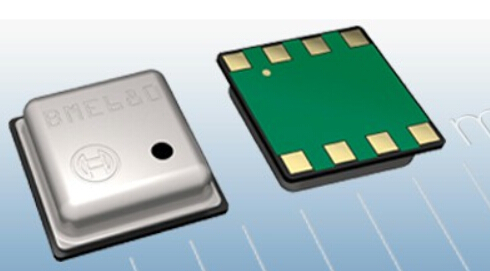
\includegraphics[width=0.35\textwidth]{Figures/Hardware/bme680_model.png}
    \caption{Capteur environnemental et qualité de l'air BME680}
    \label{fig-bme680_model}
\end{figure}

Un capteur de qualité de l'air a également été intégré sur la DevBox. Il s'agit du BME680 de Bosch Sensortec visible sur la \cref{fig-bme680_model}. Celui-ci ne mesure pas seulement la qualité de l'air, il mesure également la pression ambiante, la température, l'humidité et le gaz. Pour la mesure du gaz, il s'agit des \textit{Volatile Organic Compounds}\footnote{\url{https://en.wikipedia.org/wiki/Volatile_organic_compound}} (VOC), avec lesquels ont évalue la qualité globale de l'air ambiant. La liste des VOC utilisés pour l'index de la qualité de l'air ainsi que leur taux de précision est disponible sur la \cref{fig-bme680_voc_compounds}. Le capteur contient en interne une zone chauffante, laquelle s'active un bref instant pour pouvoir ensuite extraire la résistance de l'air. Cette résistance est la seule valeur fournie par ce capteur. Il faut ensuite faire des corrélations afin d'extraire les informations. La température, l'humidité et la pression sont elles directement retournées dans leurs unités respectives (°C, \,\% et Pa). 

\begin{figure}[ht!]
    \centering
    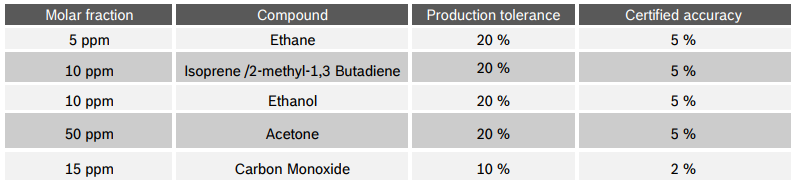
\includegraphics[width=0.8\textwidth]{Figures/Hardware/bme680_voc_compounds.png}
    \caption{VOC mesurés par le BME680}
    \label{fig-bme680_voc_compounds}
\end{figure}

Comme pour le BNO055, Bosch Sensortec met a disposition un driver en C\footnote{\url{https://github.com/BoschSensortec/BME680_driver}}. Le driver est beaucoup plus sommaire que celui du BNO055, car Bosch propose également une bibliothèque nommée BSEC pour \textit{Bosch Sensortec Environmental Cluster}\footnote{\url{https://www.bosch-sensortec.com/bst/products/all_products/bsec}}. Cette dernière n'est pas open source, il faut se contenter d'un binaire précompilé pour l'architecture utilisée. 


\subsubsection{GPS}
\label{sec-hardware_gps}

La DevBox peut également être équipée d'un GPS au besoin. Celui-ci étant assez couteux, il ne sera pas forcément monté sur toutes les cartes. Le GPS peut être utilisé si l'on souhaite traquer un objet en déplacement avec une très grande précision ($\pm$ 8m, 95\,\% du temps \cite{GPSgovGP89:online}). Il peut également être utilisé pour corréler la localisation obtenue via LoRa avec une position réelle. Cette géolocalisation par LoRa est expliquée dans l'introduction au LoRa de sous la \cref{sec_stateOfTheArtLoRa}.

\begin{figure}[ht!]
    \centering
    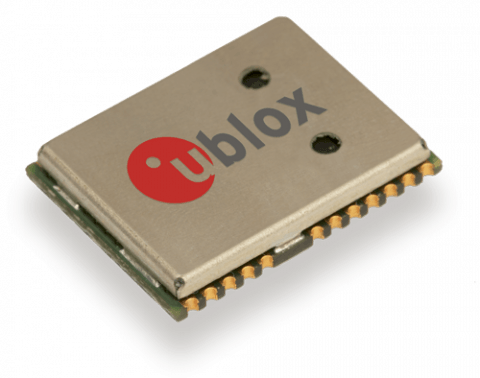
\includegraphics[width=0.35\textwidth]{Figures/Hardware/neo_3d_model.png}
    \caption{GPS U-blox NEO-M8}
    \label{fig-neo_3d_model}
\end{figure}

Le choix du GPS, a été opéré parmi ceux du fabricant suisse U-blox, spécialisé dans les semiconducteurs avec communication sans fil. Ils ont un large choix en termes de périphériques GPS. Ils proposent des GPS assortis d'antennes externes ou d'antennes céramiques placées directement sur un module. Ces GPS ont également la possibilité d'incorporer un \textit{low-noise amplifier} (LNA\footnote{\url{https://en.wikipedia.org/wiki/Low-noise_amplifier}}) pour l'amplification du signal. On peut également y trouver un filtre de type \textit{surface acoustic wave} (SAW\footnote{\url{https://www.vectron.com/products/saw/gps.htm}}) pour améliorer le signal et ainsi améliorer la réception. Lorsque ces deux éléments sont directement intégrés dans le module, cela facilite considérablement la complexité de routage d'un circuit équipé d'un GPS. En effet, s'il est nécessaire de créer ces deux éléments à l'extérieur du GPS, il faut faire particulièrement attention au type de composants utilisés, car le GPS communique à l'aide de deux hautes fréquences de 1575.42\,MHz et 1227.60\,MHz \cite{GPSsigna51:online}. Il y a également l'adaptation d'impédance sur la connexion avec l'antenne qui doit être correctement calculée en considérant l'épaisseur du circuit imprimé. \\

Le GPS recherché devait également être capable d'accepter la lecture par une interface de type I2C ou SPI, puisque ce sont les seules interfaces encore disponibles sur le KW41Z, puisque l'UART a été utilisé pour la communication entre le KW41Z et le module LoRa. Malheureusement, l'UART est l'interface la plus utilisée en GPS, donc certains GPS ne proposent que ce type de protocole de communication.

\begin{figure}[ht!]
    \centering
    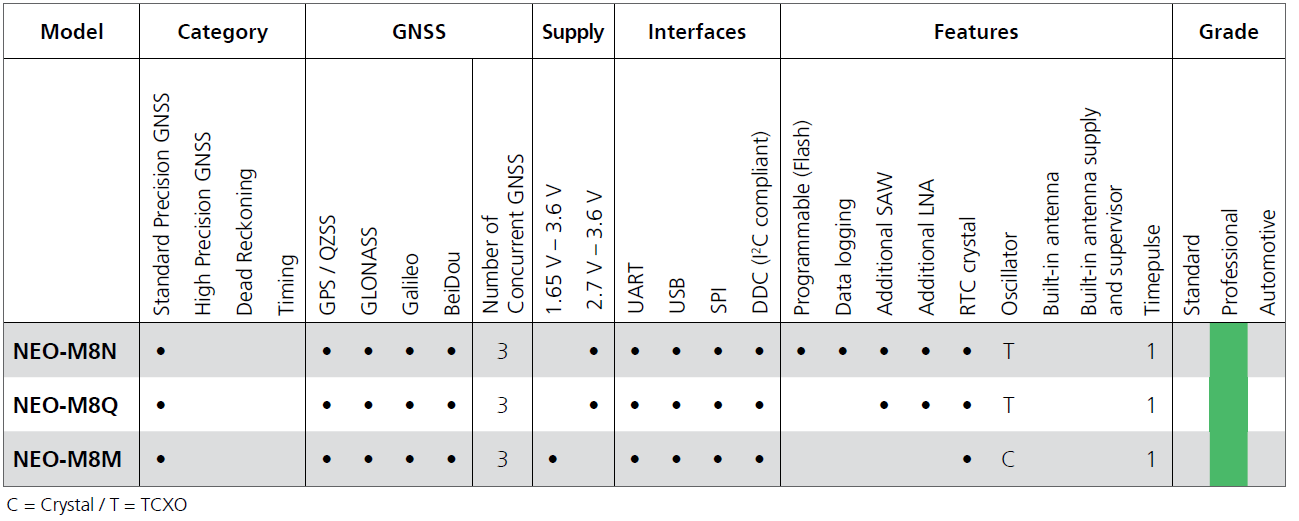
\includegraphics[width=0.95\textwidth]{Figures/Hardware/gps_neo_comparaison.png}
    \caption{Comparaison de la gamme de GPS U-blox NEO-M8}
    \label{fig-gps_neo_comparaison}
\end{figure}

Le GPS retenu a été le NEO-M8 dont la gamme complète est visible sur la \cref{fig-gps_neo_comparaison}. Celui-ci offre tout ce dont on a besoin, à savoir la possibilité d'une connexion avec une interface I2C ou SPI, ainsi que l'intégration d'un filtre SAW et d'un LNA. L'interface retenue pour le GPS a été le SPI, laquelle doit être partagée avec les composants qui sont connectés sur le connecteur PMOD (cf. \cref{sec-pmod_connector}). Sa taille est importante par rapport à celle des deux processeurs utilisés sur la carte (12.2 x 16 x 2.4\,mm pour le NEO-M8 contre 12 x 13\,mm pour le module LoRa). Il est entouré d'un boitier métallique, visible sur la \cref{fig-neo_3d_model}, afin d'atténuer les perturbations externes. Cependant, il ne nécessite aucun périphérique externe, à l'exception d'un connecteur U.FL pour la connexion d'une antenne externe.

\begin{figure}[ht!]
    \centering
    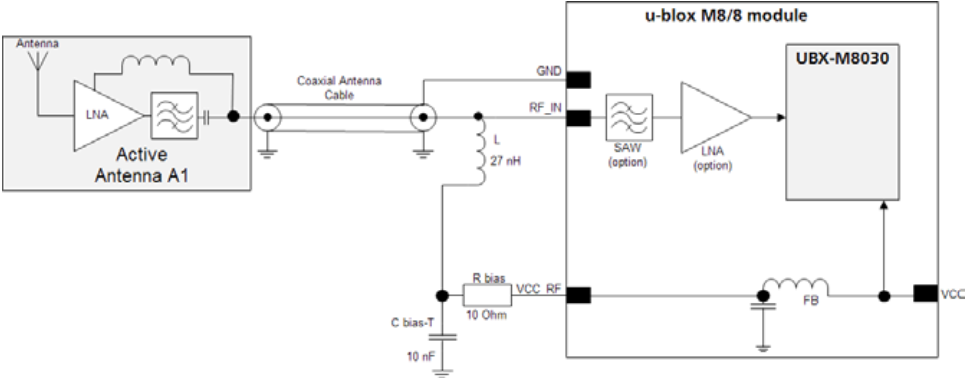
\includegraphics[width=0.9\textwidth]{Figures/Hardware/gps_neo_active_antenna.PNG}
    \caption{Schéma de connexion d'un NEO-M8 avec une antenne active}
    \label{fig-gps_neo_active_antenna}
\end{figure}

Le GPS a été routé sur la DevBox pour pouvoir utiliser des antennes non actives. Si l'utilisateur souhaite utiliser des antennes actives, il est possible de connecter l'alimentation directement le signal RF en entrée de l'antenne. Ceci n'est pas la connexion recommandée, mais elle est fonctionnelle. Selon la \textit{datasheet} du constructeur, si l'on souhaite convertir le signal RF actif, il faut normalement filtrer le signal d'alimentation afin d'éviter l'injection de bruit dans la radio. La \cref{fig-gps_neo_active_antenna} illustre la connexion recommandée par U-blox. Le NEO-M8 propose également une sortie nommée \textit{Timepulse} qui génère une pulse à chaque seconde (l'intervalle est configurable). Cette pulsation peut être utilisée pour synchroniser une horloge sur le microcontrôleur, de même que pour savoir si le GPS est prêt à fournir un nouveau paquet.\\

Ce module GPS entre directement dans la gamme professionnelle. La gamme supérieure est l'\textit{automotive} pour l'industrie des véhicules, mais il n'a pas été jugé nécessaire de prendre des composants de ce type pour le projet réalisé.
Le prix du GPS s'élève à 9.24 euros à partir de 250 pièces achetées (prix visible en janvier 2018).

\begin{figure}[ht!]
    \centering
    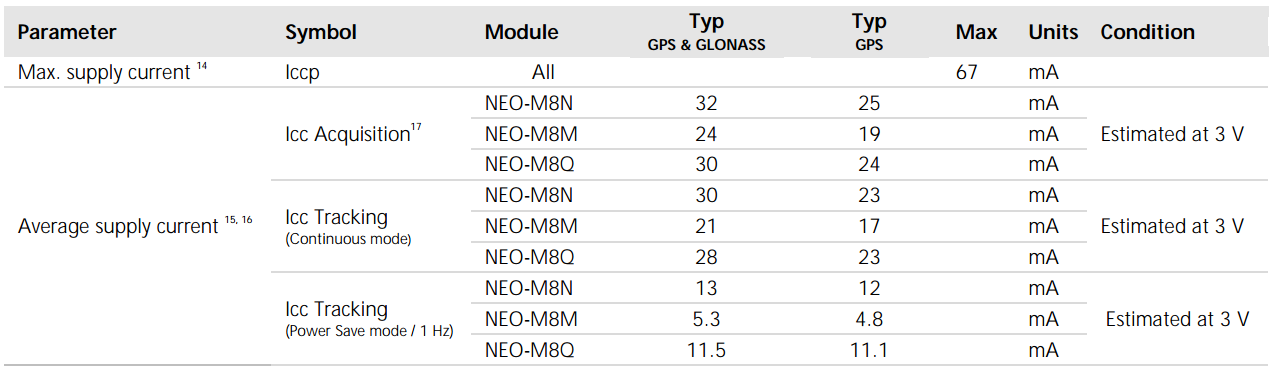
\includegraphics[width=0.95\textwidth]{Figures/Hardware/gps_neo_current_consumption.PNG}
    \caption{Consommation du GPS NEO-M8}
    \label{fig-gps_neo_current_consumption}
\end{figure}

En termes de consommation, tous les GPS sont de gourmands en énergie, car ils doivent continuer à écouter les signaux GPS. La \cref{fig-gps_neo_current_consumption} illustre combien le circuit consomme en acquisition. Cela dépend du mode choisi, le mode normal étant nommé \textit{ICC Acquisition}. Pour le NEO-M8Q, la consommation est en moyenne de 30mA avec GLONASS et GPS utilisés. À cette consommation, il faut encore ajouter celle d'une antenne active, dans la mesure où ce type d'antenne est raccordée. Les antennes actives consomment entre 3mA et 25mA selon les modèles utilisés. La consommation finale oscille ainsi autour de 50 mA, ce qui est problématique pour beaucoup de systèmes embarqués autonomes. Heureusement, le NEO-M8 peut être placé en mode \textit{low-power} via l'utilisation de commandes UBX; il est toutefois impossible de trouver la valeur exacte de la consommation de ce mode parmi les documents de U-blox. La seule référence à la consommation indique ce qui suit : 

\begin{quote}
\begin{center}
    \textit{During operation, the current drawn by the module can vary by some orders of magnitude, especially if enabling low-power operation modes.}
\end{center}
\end{quote}

Aucune valeur n'est fournie pour la consommation dans ce mode. Il est également possible de placer le GPS en mode \textit{backup}. C'est un mode où le GPS est désactivé, mais l'éphéméride des satellites est sauvegardée dans une mémoire volatile pour accélérer la synchronisation lorsque le mode normal est resélectionné. Pour sauver l'état de cette mémoire, une tension doit être appliquée au circuit sur une pin spécifique. Cette sauvegarde consomme 15\si{\micro{}}A si la tension de l'alimentation est de 1.8V. Ce type de mémoires peuvent être alimentées par des piles boutons, puisque le seuil minimum de tension est de 1.4V. Dans le cadre de ce projet, cette pin a été directement connectée à la tension VCC du circuit, celui-ci étant régulé par une batterie.


\subsubsection{Connecteur PMOD}
\label{sec-pmod_connector}

La carte DevBox est également compatible avec les connecteurs PMOD. Ces connecteurs sont basés sur un standard d'interface\footnote{\url{https://en.wikipedia.org/wiki/Pmod_Interface}} du même nom développé par l'entreprise Digilent\footnote{\url{http://store.digilentinc.com/}}. Le pinout des différents types d'interfaces est disponible sur la \cref{fig-pmod_type_pinout}. Dans le cas de la DevBox, les standards n'ont malheureusement pas pu être intégralement respectés, en raison de l'absence de GPIO disponibles sur le module Bluetooth. Les connecteurs sont compatibles avec les PMOD de type I2C, à l'exception des deux IO et des signaux. L'interface SPI est supportée à l'exception de INT et RST. Le pinout final de la DevBox est visible sur le schéma \texttt{PMOD} de l'\cref{AppendixDevBoxHardware}.\\

\begin{figure}[ht!]
    \centering
    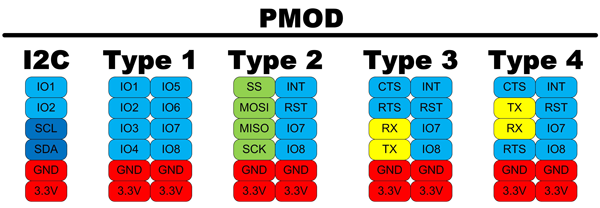
\includegraphics[width=0.7\textwidth]{Figures/Hardware/pmod_type_pinout.png}
    \caption{Pinout du standard PMOD en fonction des types choisis}
    \label{fig-pmod_type_pinout}
\end{figure}

Digilent commercialise des modules compatibles avec ces interfaces, ce qui facilite l'ajout d'un type de capteur qui n'aurait pas , par défaut, été rajouté sur la carte de développement. Le problème lié aux processeurs utilisés est le nombre de connexions disponibles vers l'extérieur. Nos deux microcontrôleurs ne sont équipés que de 48 pins au total, dont la moitié sont utilisés pour les alimentations et divers contrôles internes.

\FloatBarrier


\section{Schéma bloc général final}


La \cref{fig-hardware_bloc_diagram} illustre le schéma bloc final sur Altium de la carte DevBox. Il représente toutes les interfaces de communications entre les différents blocs. Cette image est également disponible sur l'\cref{AppendixDevBoxHardware}, tout comme les autres schémas électroniques du projet.\\


\begin{figure}[ht!]
    \centering
    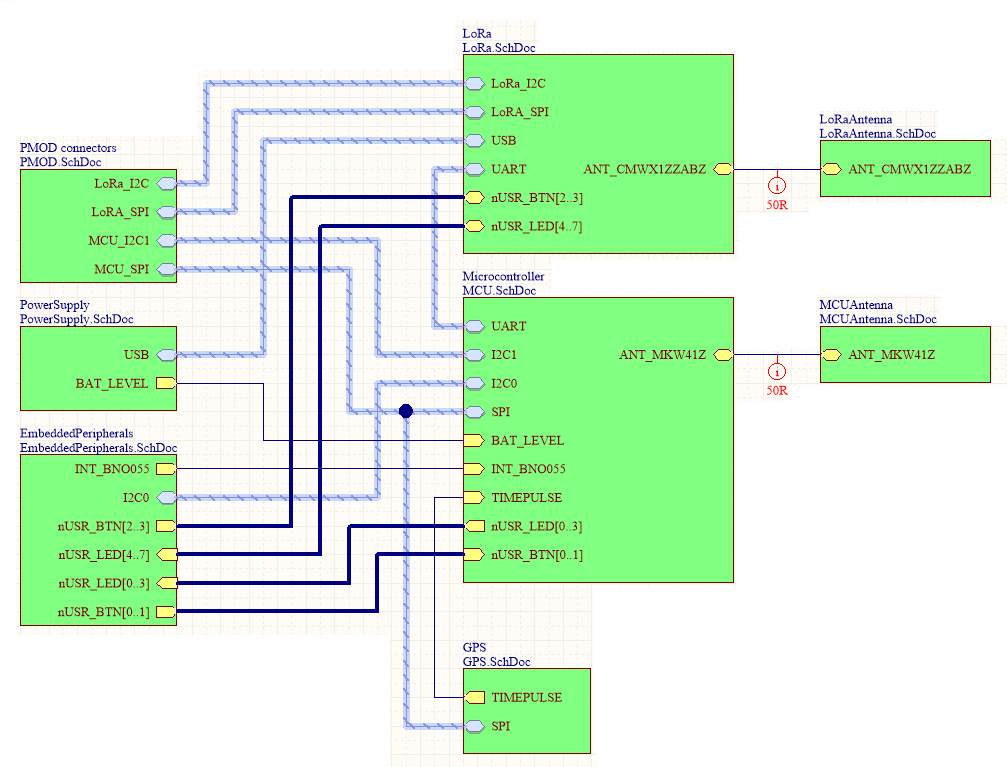
\includegraphics[width=1.05\textwidth]{Figures/Hardware/hardware_bloc_diagram.png}
    \caption{Schéma bloc général de la DevBox}
    \label{fig-hardware_bloc_diagram}
\end{figure}


\FloatBarrier
\section{Réalisation et production du circuit électronique}

Le PCB réalisé a été routé selon les contraintes du fabricant de PCB\footnote{\url{https://www.pcbway.com/}} choisi, soit PcbWay. L'épaisseur choisie est de 1.6mm et les largeurs de piste minimales de 4mil. Les plus petits trous autorisés sont de 0.2mm. Afin de facilité la soudure, une finition à l'or a été demandée. Le temps de production est d'environ une semaine et demie à partir du moment où la transaction est validée. \\

Les composants électroniques ont principalement été commandés auprès de trois fournisseurs: Mouser, Farnell et Digikey. Mouser a été privilégié pour les composants, les deux autres n'ayant été utilisés qu'en cas de rupture de stock chez Mouser. La liste complète des composants avec leurs numéros de commande sont indiqués dans le projet Altium présent sur GitHub.\\

Un masque de dépose de pâte a dû être commandé à l'entreprise DB Products\footnote{\url{https://www.dbproducts.fr/}}. Une fois celui-ci reçu la production a pu être effectuée avec une machine de dépose de composants manuelle.

\section{Erreurs de conception et corrections possibles}
\label{sec_hardware_errors}

Une fois le PCB réalisé, plusieurs tests ont été effectués pour vérifier son fonctionnement. Quelques erreurs critiques ont du être corrigées : 

\begin{itemize}
    \item \textbf{Module LoRa} : VDD\_USB doit être connecté au 3.3V et non au 5V;
    \item \textbf{Module LoRa/Bluetooth} : RX et TX sont inversés sur la ligne UART;
    \item \textbf{Module LoRa} : VDD\_TCXO doit être connecté à la pin PA12 afin de pouvoir placer le SX1276 en mode \textit{sleep}.\\
\end{itemize}

Quelques améliorations peuvent également être envisagées pour la prochaine version, celles-ci n'étant toutefois pas un obstacle au fonctionnement de la version actuelle de la DevBox : 

\begin{itemize}
    \item \textbf{Module LoRa} : Connecter la mesure de la batterie (diviseur de tension) sur une pin ADC du module LoRa. Pour ce faire, il faut également relier la pin VREF à une référence externe ou au VCC. A l'heure actuelle, uniquement le KW41Z a accès à cette mesure.
    \item \textbf{GPS} : Ajouter le support d'une antenne active sur le PCB avec l'ajout de la tension d'alimentation filtrée sur le signal RF. Il est également possible d'ajouter un autre LNA à la sortie du signal RF (cf. \texttt{Hardware Integration} PDF aux pages 15 et 16). 
    \item \textbf{GPS} : Si l'on souhaite mettre en veille le GPS, il est possible de configurer une pin afin que celle-ci le place en mode \textit{sleep} lorsqu'elle est placée à un état 0. Il s'agit là de la pin EXTINT, mais celle-ci doit préalablement être programmée au moyen du protocole UBX.
    \item \textbf{GPS} : Connecter la pin GPS\_nCS sur une pin contrôlable par le DSPI en tant que \textit{chip select}. Actuellement, cette pin est contrôlée par un GPIO.
    \item \textbf{PCB layout} : Déplacer le bouton reset du KW41Z afin d'éviter les \textit{resets} non souhaités lors de la connexion sur câble JTAG. 
    \item \textbf{PCB layout} : Placer les boutons du KW41Z en face des LED du même microcontrôleur.
    \item \textbf{PCB layout} : Les LED de la charge de la batterie peuvent être placées sur le haut de la carte.
    \item \textbf{BME680} : Le BME680 pourrait être placé dans un coin plus proche du bord de la carte. On peut également découper un sillage autour du capteur afin de limiter la chauffe du PCB.
\end{itemize}

\section{Boitier en plastique}

\begin{figure}[ht!]
    \centering
    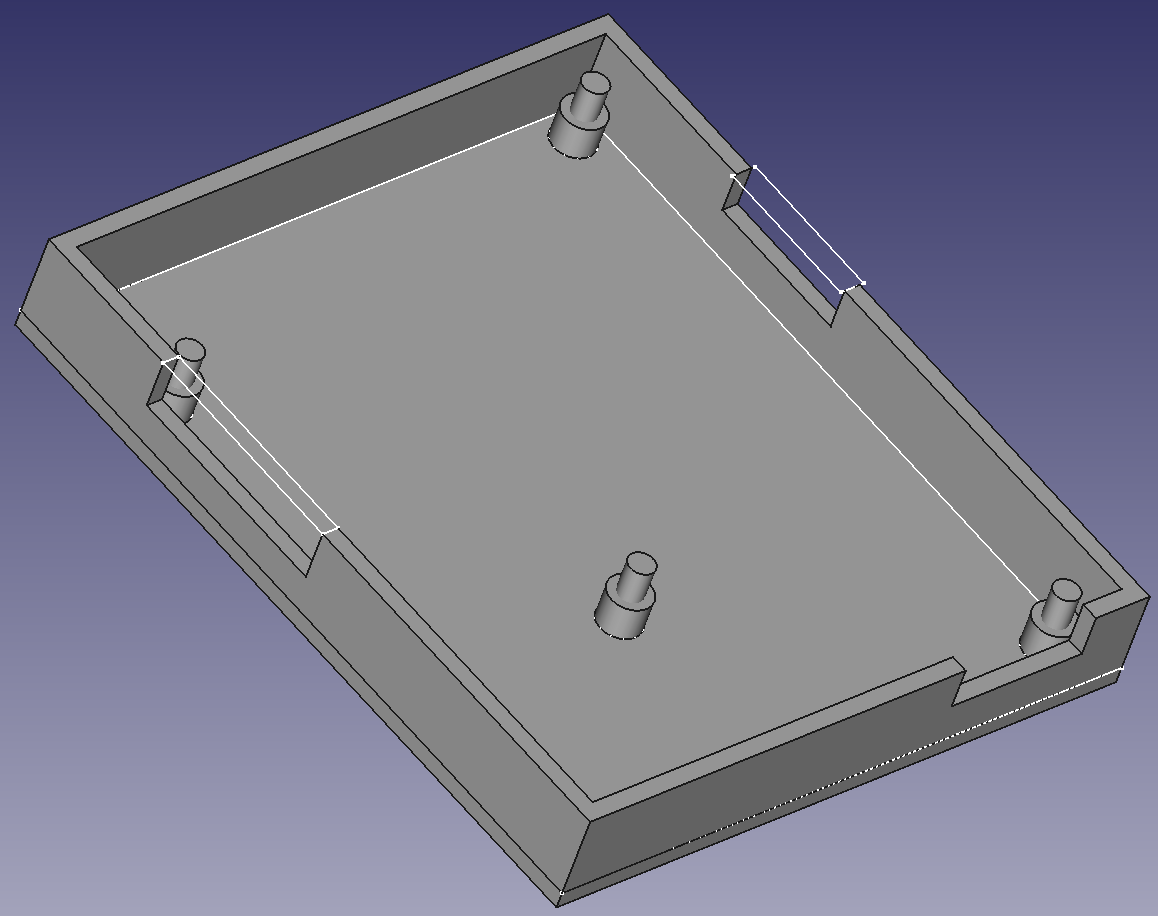
\includegraphics[width=0.6\textwidth]{Figures/Hardware/3d_case_devbox.png}
    \caption{Boitier imprimé en 3D pour y loger le circuit électronique}
    \label{fig-3d_case_devbox}
\end{figure}

Un petit boitier en plastique, visible sur la \cref{fig-3d_case_devbox}, a été créé afin d'y loger la carte. Ce boitier a été réalisé à l'aide du logiciel freecad\footnote{\url{https://www.freecadweb.org/}} et est cité dans les sources du projet sur GitHub. Son impression a été réalisée à l'aide d'une imprimante 3D.



\FloatBarrier

